% !TeX spellcheck = en_US

\chapter{Theoretical and Experimental Results}
\section{Training data}
For the training, we wanted to use publicly and freely available data, which lead to Open Street Map for the vector data and Microsoft Bing Maps for the imagery. A dataset consisting of satellite imagery and images for the ground truths can be created using the Python module Airtiler \cite{airtiler}.

Furthermore, there are several different datasets publicly available: \cite{VolodymyrMnih.2013}, \cite{spacenet}, \cite{isprs-vaihingen}, \cite{isprs-potsdam}, \cite{Helber.20170831}, \cite{deepsat}.

\section{Microsoft COCO}
For the crowdAI Mapping Challenge \cite{mappingchallenge} the instances were represented in the Microsoft COCO annotation format \cite{cocoformat}. Unfortunately, using this format, it is not possible to represent polygons with holes in it\footnote{\url{https://github.com/cocodataset/cocoapi/issues/153, 21.05.2018}}. As there are many buildings, for which this would be required, we decided not to use this format and instead use images for the representation of the ground truths.

\begin{figure}[H]
	\centering
	\begin{subfigure}{0.4\textwidth}
		\centering
    	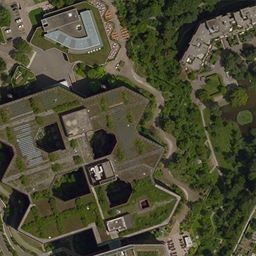
\includegraphics[width=0.9\linewidth]{chapters/theoretical_and_experimental_results/images/building_with_hole.png}		    \caption{A building with multiple holes}
	\end{subfigure}~
		\begin{subfigure}{0.4\textwidth}
		\centering
    	
\includegraphics[width=0.9\linewidth]{chapters/theoretical_and_experimental_results/images/building_with_hole_gt.png}		    \caption{Predicted building masks}
	\end{subfigure}
	\caption{The corresponding ground truth}
	\label{fig:results:buildings_with_holes_gt}
\end{figure}

\section{Building detection}
tbd

\section{Mapping Challenge}
At the time of this writin the platform crowdAI hosted a challenge called Mapping Challenge \cite{mappingchallenge} which was about detecting buildings from satellite imagery. In order to gain additional knowledge regarding the performance of Mask R-CNN, we decided to participate in the challenge.

\autoref{tab:results:mapping_challenge_results} shows the changes made to the Mask R-CNN config and their impact on the prediction accuracy.

\newcolumntype{b}{>{\hsize=2.3\hsize}X}
\newcolumntype{s}{>{\hsize=.5\hsize}X}
\newcolumntype{m}{>{\hsize=.9\hsize}X}

\begin{table}[t]
\begin{tabularx}{\textwidth}{sssbss}
    \# Epochs & \# Steps / Epoch & \# Validation Steps & Config Change & AP@0.5 & AR@0.5 \\  \midrule
100 & 2500 & 150 & - & 0.798 & 0.566 \\ 
100 & 2500 & 150 & Image mean RGB updated & 0.799 & 0.564 \\ 
100 & 2500 & 150 & Mini mask disabled & 0.807 & 0.573 \\ 
100 & 5000 & 200 & + validation steps & 0.821 & 0.599 \\ 
100 & 10000 & 200 & + steps / epoch & 0.833 & 0.619 \\ 
100 & 20000 & 300 & + Validation steps, + steps / epoch & 0.853 & 0.885 \\  \bottomrule
\end{tabularx} 
    \caption{Mapping challenge results}
    \label{tab:results:mapping_challenge_results}
\end{table}

Generally, these results indicate, that finetuning of hyperparameters has an impact. Furthermore, the even bigger impact can be made just by longer training. However, in case of longer training, one has to make sure, that the network will not overfit. In the case of an already existing architecture like Mask R-CNN for example, this has already been done. On the other hand, if one develops a new architecture, overfitting has to be taken care of, for example with a technique called Dropout \cite{Srivastava.2014}. Generally, Dropout randomly disables some units during the training. As a result of this, the model constantly changes and overfitting can not happen that easily.